\documentclass[output=paper,colorlinks,citecolor=brown,footheight=42pt]{langscibook}
\ChapterDOI{10.5281/zenodo.12090441}
\author{Terje Lohndal\affiliation{NTNU – Norwegian University of Science and Technology; UiT The Arctic University of Norway} and Michael T. Putnam\affiliation{Penn State University;University of Greenwich (CREL)}\orcid{}}

\title{Expanding structures while reducing mappings: Morphosyntactic complexity in agglutinating heritage languages}

\abstract{Research on heritage language grammars to date provides overwhelming support for the general stability of their syntactic systems, while the status of their morphology can vary considerably. In this chapter we offer remarks on the morphological complexity of agglutinating heritage languages, taking a closer look at a number of phenomena in Labrador Inuttitut, Cherokee, and American Hungarian. Four important findings emerge from our review: First, these phenomena align with previously documented and observed patterns in heritage language morphology \citep{polinsky2018heritage,putnametal2021}. Second, heritage language morphology maintains a significant degree of complexity, even in languages found to be in a moribund state \citep{bousquette2020}. Third, adopting an exoskeletal approach to morphosyntactic decomposition and complexity \citep{lohnput21}, we observe trends towards larger syntactic structures (for lexicalization), and inversely a reduction in the inventory of exponency. Fourth, we observe a general trend in the “shrinking” of computational domains for lexicalization and movement operations.}



\IfFileExists{../localcommands.tex}{%hack to check whether this is being compiled as part of a collection or standalone
   \usepackage{tabularx,multicol}
\usepackage{url}
\urlstyle{same}
\usepackage{multirow}

\usepackage{stmaryrd}
\usepackage{soul}
\usepackage{enumitem}

\usepackage{siunitx}
\sisetup{group-digits=none}

\usepackage{langsci-optional}
\usepackage{langsci-lgr}
\usepackage{langsci-textipa}
\usepackage{langsci-branding}

\usepackage{tikz-qtree}

\usepackage{pgfplots}
\usepackage{qtree}
\qtreecenterfalse
\usepackage{tree-dvips}
\usepackage{subcaption}

\let\clipbox\undefined
\usepackage{adjustbox}
\usepackage[linguistics, edges]{forest}
\usepackage{langsci-gb4e}

% ORCIDs in langsci-affiliations 
\usepackage{orcidlink}
\SetupAffiliations{orcid placement=before}
\definecolor{orcidlogocol}{cmyk}{0,0,0,1}
\RenewDocumentCommand{\LinkToORCIDinAffiliations}{ +m }
  {%
    \orcidlink{#1}\,%
  }

   \newcommand*{\orcid}[1]{}


\makeatletter
\let\thetitle\@title
\let\theauthor\@author
\makeatother

\newcommand{\togglepaper}[1][0]{
   \bibliography{../localbibliography}
   \papernote{\scriptsize\normalfont
     \theauthor.
     \titleTemp.
     To appear in:
     E. Di Tor \& Herr Rausgeberin (ed.).
     Booktitle in localcommands.tex.
     Berlin: Language Science Press. [preliminary page numbering]
   }
   \pagenumbering{roman}
   \setcounter{chapter}{#1}
   \addtocounter{chapter}{-1}
}

\newbool{bookcompile}
\booltrue{bookcompile}
\newcommand{\bookorchapter}[2]{\ifbool{bookcompile}{#1}{#2}}


\forestset{
  my nice empty nodes/.style={% modified from manual page 52
    for tree={
      calign=fixed edge angles,
      calign angle=50,
    },
    delay={
      where n children=0{
        if content={}{
          content=\strut,
          anchor=north,
        }{
          align=center
        },
      }{
        if content={}{
          shape=coordinate,
          for parent={
            for children={
              anchor=north
            }
          }
        }{}
      }
    },
  },
  my pretty nice empty nodes/.style={
    for tree={
      calign=fixed edge angles,
      calign angle=50,
      parent anchor=south,
      delay={
        where n children=0{
          if content={}{
            content=\strut,
            anchor=north,
          }{
            align=center
          },
        }{
          if content={}{
            inner sep=0pt,
            edge path={\noexpand\path [\forestoption{edge}] (!u.parent anchor) -- (.south)\forestoption{edge label};}
          }{}
        }
      }
    }
  }
}


\newcommand{\sem}[1]{\mbox{$[\![$#1$]\!]$}}
\newcommand{\type}[1]{\ensuremath{\left \langle #1 \right \rangle }}
\newcommand{\lam}{\ensuremath{\lambda}}
\renewcommand{\and}{$\wedge$ }
\newcommand{\bex}{\begin{exe}}
\newcommand{\eex}{\end{exe}}
\newcommand{\bit}{\begin{itemize}}
\newcommand{\eit}{\end{itemize}}
\newcommand{\ben}{\begin{enumerate}}
\newcommand{\een}{\end{enumerate}}

\newcommand{\gcs}[1]{\textcolor{blue}{[gcs: #1]}}
\newcommand{\ash}[1]{\textcolor{orange}{[ash: #1]}}
\newcommand{\ngn}[1]{\textcolor{purple}{[ngn: #1]}}

\newcommand{\firstrefdash}{}


\forestset{
fairly nice empty nodes/.style={
delay={where content={}
{shape=coordinate, for siblings={anchor=north}}{}},
for tree={s sep=4mm}
}
}



   %% hyphenation points for line breaks
%% Normally, automatic hyphenation in LaTeX is very good
%% If a word is mis-hyphenated, add it to this file
%%
%% add information to TeX file before \begin{document} with:
%% %% hyphenation points for line breaks
%% Normally, automatic hyphenation in LaTeX is very good
%% If a word is mis-hyphenated, add it to this file
%%
%% add information to TeX file before \begin{document} with:
%% %% hyphenation points for line breaks
%% Normally, automatic hyphenation in LaTeX is very good
%% If a word is mis-hyphenated, add it to this file
%%
%% add information to TeX file before \begin{document} with:
%% \include{localhyphenation}
\hyphenation{
    par-a-digm
    peri-phras-tic
    mor-pho-pho-nol-o-gy
}

\hyphenation{
    par-a-digm
    peri-phras-tic
    mor-pho-pho-nol-o-gy
}

\hyphenation{
    par-a-digm
    peri-phras-tic
    mor-pho-pho-nol-o-gy
}

    \bibliography{localbibliography}
    \togglepaper[23]
}{}


\begin{document}
\shorttitlerunninghead{Expanding structures while reducing mappings}
\maketitle

\section{Introduction}
Morphology proper has been -- and continues to be -- a hotly contested and embattled domain of linguistic inquiry. One particular debate in which morphology tends to rear its (ugly) head time and again centers on attempts to determine and measure \textit{complexity} in linguistic systems. Of course, an unavoidable prerequisite to any of these arguments requires the establishment of two important points:
(1) exactly \textit{how}, i.e., according to what set of heuristics, one intends to measure complexity/simplicity, and
(2) exactly \textit{where} morphological processes and operations are located within a particular architecture, i.e., is morphology afforded a unique modular status or is it distributed across other modules? Speaking to the first point, arriving at an agreed upon metric to measure morphological complexity has proven to be quite elusive \citep{arkadiev2020,stump2017,anderson2015}, with some linguists resorting to frequency and entropy conditions \citep{ackerman2013}, while others turn to particular processes, such as \textit{demorphologization}, as a sign of an increase (or decrease) in systemic morphological complexity \citep{mansfield2020,hopper1990}. An outcome of this research that bears repeating is that complexity in detailed and accurate description extends beyond inflectional morphology and may reach all the way into syntax. The lack of a universally agreed upon complexity metric in connection with morphology spills over into theory-building efforts \citep{mithun2020}. In this chapter, we adopt the approach that the division between “morphology” and “syntax” is largely arbitrary \citep{haspelmath2011}, and further develop a model of morphological complexity in heritage language grammar initially sketched out by \citet{lohnput21}.\largerpage


An additional confound arises when we analyze the morphology of bi- and multilinguals, and heritage bilinguals in particular. Experimental research overwhelmingly confirms the integrated nature of the bilingual lexicon \citep{kroll2014speech,PutnamEtAl2018}. The current consensus seems to advocate a general reduction in complexity in heritage morphology \citep{scontras2015,ScontrasEtAl2018}, and some argue that these outcomes are an indication of different developmental trajectories in heritage language morphology \citep{berdicevskis2020}. In spite of the suggested trend towards “simplification” (again, however one determines to measure this out), it is difficult, and in some instances even erroneous, to insinuate that (some level) of complexity is not maintained in heritage language grammars. Evidence in support of this claim can be found in moribund heritage grammars \citep{bousquette2020} as well as in the grammar of receptive bilinguals \citep{sherkinalieber2015}.   
In this chapter we take a closer look at the concept of morphological complexity in a particular set of heritage languages, namely, those that can be typologically classified as being \textit{agglutinating}. In the remainder of this paper, we classify \textit{polysynthetic} languages as a sub-class of agglutinating ones.{\interfootnotelinepenalty=10000\footnote{Polysynthetic languages are by nature somewhat difficult to disambiguate from agglutinating ones \citep{baker1996,mattissen2004structural}, however, one key trait that these former languages exhibit in more detail than the latter is complex phonological alternations in addition to agglutination.}} 

Although it has been suggested that irrespective of their typological distinction, the morphology of heritage bilinguals seems to follow a limited number of observable, perhaps \textit{universal} trends \citep{polinsky2018heritage,PolinskyScontras2020,putnametal2021}, there are two structural outcomes in particular that we would like to examine in more detail. The first of these involves the “teasing apart” of synthetic morphological forms in favor of more analytic forms. Consider the following data from the polysynthetic heritage language Caddo (from \citealt[74]{chafe76}, cited by \citealt[5--6]{melnar2005}). The examples in (\ref{goodCaddo}) involve posture stative predicates, which are expressed as single, morphologically complex units (or, \textit{words}). 

\begin{exe}

\ex \label{goodCaddo}

\begin{xlist}

\ex \gll háhʔ\textbf{awisʔ}nássaʔ \\
\textsc{ind}-sitting-be.cold-\textsc{impfv} \\
\glt `[he] is cold while sitting.' 

\ex \gll háhʔ\textbf{ánkisʔ}nássaʔ \\
\textsc{ind}-standing-be.cold-\textsc{impfv} \\
\glt `[he] is cold while standing.' 

\ex \gll háhʔ\textbf{ini}.nássaʔ \\
\textsc{ind}-lying-be.cold-\textsc{impfv} \\
\glt `[he] is cold while lying.' 

\end{xlist}

\end{exe}

\noindent
\citet{chafe76} reported that expressing the posture stative predicates \textit{ʔawis-} `sitting', \textit{ʔanikis-} `standing', and \textit{ʔini-} `lying' can now only be expressed by periphrastic counterparts, with the verbal element combined with a following copula. These structures consist of two \textit{words} rather than just one, see (\ref{badCaddo}).


\begin{exe}

\ex \label{badCaddo}

\begin{xlist}

\ex \gll háhʔánássaʔ háhʔ\textbf{áwsaʔ} \\
\textsc{ind}-be.cold-\textsc{impfv} \textsc{ind}-sitting-be \\
\glt `[he] is cold while sitting.' 

\ex \gll háhʔánássaʔ háhʔ\textbf{ánkisaʔ} \\
\textsc{ind}-be.cold-\textsc{impfv} \textsc{ind}-standing-be \\
\glt `[he] is cold while standing.' 

\ex \gll háhʔánássaʔ
háhʔ\textbf{\'{i}nʔaʔ} \\
\textsc{ind}-be.cold-\textsc{impfv} \textsc{ind}-lying-be \\
\glt `[he] is cold while lying.' 

\end{xlist}


\end{exe}

\noindent
The second structural property of agglutinative heritage languages that we consider here are cases whereby morphological exponents can be used in a wider set of contexts than before. As such, these exponents have a more generalized meaning and they have lost the connection to the previously specified meaning. For now, we refer to such elements as \textit{generalized exponence}. As an example of this, consider noun stems in Upper Tanana derived by the suffix \textit{\textltilde}. Many of the nouns denoting tools and instruments contain this morpheme, whose instrumental meaning in the heritage language has become opaque or lost in most instances (data from \citealt[148]{lovick2020}).

\begin{exe}

\ex \label{uppertanana} Upper Tanana noun stems derived with \textit{\textltilde}

\begin{xlist}

\item \textit{tee\textit\textltilde} `mat' 

\item \textit{ee\textit{\textltilde}} `trap' 

\item \textit{tsii\textit{\textltilde}} `bridge', `weir' 

\end{xlist}

\end{exe}

\begin{sloppypar}\noindent
These morphological processes raise interesting and timely questions for linguists interesting in gaining a better understanding of the formal properties of complexity in heritage language morphology.\footnote{Note that we are here treating indigenous languages and immigrant languages on a par. In terms of formal properties, we believe that this can be justified, although this of course does not entail that the community dynamics of these contexts do not often differ substantially.} The first involves cases whereby morphemes are ``decoupled” from their original host, leading to \textit{increased analyticity} \citep[183]{polinsky2018heritage}. This state of affairs suggests that some degree of relativized economy of representations may also be present \citep{scontras2015,ScontrasEtAl2018,perezc2019,PolinskyScontras2020,putnametal2021}. The second scenario reveals the opposite trend, namely, the maintenance of morphological forms that have become, or are well on their way to becoming, semantically bleached. Here we examine these trends in agglutinating heritage languages with consideration of how these contribute to a unified narrative on complexity in heritage grammars.
\end{sloppypar}

As already noted, in this chapter we home in on properties and trends observed in the morphology of \textit{agglutinating} heritage languages, with a particular focus on verbal elements. Two of the three languages reviewed are also polysynthetic. In \sectref{common} we briefly review common properties of heritage morphology that transcend typological class \citep{polinsky2018heritage,putnametal2021}. We introduce our formal conceptualization of complexity in \sectref{formalcomplexity}, building on an initial treatment set forth by \citet{lohnput21}. In \sectref{verbsection} we sketch out an analysis of aspects of verbal morphology of heritage Inuttitut, Cherokee, and American Hungarian, focusing on the the rise of \textit{increased analyticity} (\sectref{analsub}) and \textit{generalized exponence} (\sectref{weaksub}) and how their presence contributes to our treatment of complexity in heritage languages at the syntax-morphology interface. We provide the sketch of an analysis of these tendencies in \sectref{decompose}, showing how an exoskeletal approach to the morphology-syntax interface delivers a unique and promising perspective on addressing the notion of complexity in heritage languages. Finally, we conclude this chapter in \sectref{outro}, pointing out fruitful areas of research into the notion of (morphological) complexity in heritage language grammars.

\section{Structural tendencies in heritage morphology} \label{common}
As discussed in detail by \citet[Ch. 5]{polinsky2018heritage} and \citet[\S 2]{putnametal2021}, the morphological systems of heritage languages share a number of structural tendencies. Space and time prevent us from providing a comprehensive overview of these common traits, however, we do wish to highlight both these general trends and additionally what they mean for establishing a formal heuristic of complexity. Morphological systems found in heritage languages develop a propensity for one-structure-to-one-meaning mappings irrespective of the typological system of morphology a particular language (predominantly) adheres to. Still, as we discuss in the remainder of this paper, there are interesting puzzles that heritage languages with agglutinating and polysynthetic morphological systems pose for attempts to formalize notions of representational economy and complexity. 

\citet{putnametal2021} identify five primary patterns observed in heritage morphology irrespective of typological classification: (i) transparency and salience of forms and structures, (ii) overregularization and overmarking, (iii) preference for analytical forms, (iv) avoidance of ambiguity and underspecification, and (v) minimal domains. Let us now discuss each of these in turn based on the discussion in \citet{putnametal2021}, which the reader should consult for examples and references.

Transparency of forms and structures refers to the mapping between an underlying feature and a given exponent. The most transparent case is the case whereby one feature refers to one exponent, making both readily identifiable. Therefore, forms and structures that are transparent are easier to detect in complex morphological paradigms. Typically, transparent forms will win out at the expense of less transparent forms. One illustration of this comes from grammatical gender, where heritage speakers often struggle to assign grammatical gender to non-transparent nouns. Another one involves the complete loss of a structural form, which has been found, e.g., for the subjunctive.

Overregularization occurs when a speaker overuses highly transparent and regularized forms. For example, a particular morphological case form may be overextended and generalized so that, say, the nominative is also used with direct objects. When other case features are lost, the nominative form becomes more accessible and therefore easier to overuse. However, it is not the case that what is robust in the input is always retained in heritage grammars. Subject-verb agreement is a good example, which often is reported to be vulnerable despite its prevalence in the input. Overmarking, on the other hand, is argued by \citet{putnametal2021} to be a special case of overregularization whereby a particular form is used in contexts where it normally would not be used. An example from \citet{polinsky2018heritage} involving heritage English is the overuse of the weak past tense {\itshape -ed} marker, producing forms such as {\itshape dresseded, walkeded,} {\itshape sanged,} and {\itshape wented}. That is, the weak past tense form is overmarked.

Turning to the preference for analytical forms, this refers to the preference for analytical and periphrastic forms compared to synthetic ones. We saw an example of this already in the introduction. This may come from a drive to establish one-to-one mappings between form and meaning, which in turn will provide more transparent mappings (cf. the first pattern). Ultimately, this preference may be due to a bias in children to assume a one-to-one mapping between form and meaning when acquiring a language, cf. \citet{slobin1973} and \citet{vanHout2008}. If so, it is no surprise that such a bias is accentuated in heritage language settings  \citep{polinsky2018heritage}.

A consequence of the preference for one-to-one mappings is the preference in heritage speakers to avoid structural ambiguities. That is, speakers avoid instances where one form may be associated with different meanings. For instance, in languages with dative case, due to the multiplicity of functions and mappings of dative case, restructuring is prone to occur. Assuming that scope is structurally determined, another illustration is that speakers tend to go for surface scope readings as opposed to inverse scope ones. Furthermore, heritage speakers tend to avoid underspecification in cases where two or more segments form a paradigmatic opposition. Instead, they often go for fully valued features, in which case oppositions act as a “vaccine” against underspecification. Generally, heritage speakers opt for one pattern or a fully specified feature structure.

The last pattern is what is typically referred to as {\itshape minimal domains}. This refers to a preference for minimal domains of computation. For instance, adjacent forms are preferred over dependencies that span a distance. In more formal terms, this suggests that the domains of computation are somehow “smaller” in heritage grammars. One way in which this occurs is for example by a reduction in the functional spine, either through heads/features merging or through a head/feature being eliminated.

With these five patterns in mind, we next turn to an attempt to decompose the notion of complexity and thereby put it on a more formal grounding. 

\section{Formalizing complexity} \label{formalcomplexity}
As \citet{lohnput21} demonstrate, complexity has been a much discussed topic in general and in the context of heritage grammars. The general intuition has been that heritage grammars tend to exhibit reduced complexity, although as Lohndal \& Putnam also point out, complexity is a much too coarse grained notion to be of much use in understanding the nature of heritage grammars. Instead, it is vital to decompose {\itshape complexity} into familiar concepts and notions. In this section, we will summarize the approach developed in \citet{lohnput21}, where three concepts are central in modeling complexity in a formal system.

\begin{exe}
\item Criteria for establishing complexity: \label{criteria}
\begin{xlist}
\item Number of syntactic features
\item Number of functional projections
\item Mapping from syntactic features to exponents
\end{xlist}
\end{exe}

The criteria in  (\ref{criteria}) require a decompositional approach to the lexicon and an architecture which clearly distinguishes between syntax proper and morphophonology. A general label for such approaches is {\itshape exoskeletal approaches}, that is, approaches whereby syntactic structures determine both grammatical properties and “the ultimate fine-grained meanings of lexical items themselves" \citep[33]{borer2003}.\footnote{We won't provide an in-depth discussion of the relative merits of exoskeletal approaches over endoskeletal approaches. Readers are referred to, among many, \citet{borer2005nouns, borer2005events, lohndal2014, lohndal2019} and \citet{wechsler2021} for discussion.} Unlike many traditional approaches whereby lexical items feed syntactic operations, syntactic structures are built from atomic features which are then associated with morphophonological realizations. The latter invokes a realizational approach to morphology in which morphosyntactic properties determine inflectional morphemes (see \citealt{stump2001} for more on this). The syntax consists of atomic units, often referred to as roots and formal features, which mark syntactic and semantic properties. In turn, these map onto morphophonological realizations, called {\itshape exponents}. This mapping is subject to controversy, with proposals ranging from Distributed Morphology \citep{halle1993} to Nanosyntax \citep{starke2009}. We will briefly review each of these approaches.

Within Distributed Morphology, a Vocabulary Item denotes the mapping between abstract features and exponents. This is illustrated in (\ref{vocabitem}) (adopted from \citealt[9]{embick2015}):

\begin{exe}
\ex \label{vocabitem} Vocabulary Item
\begin{tabular}{ccc}
$[\alpha\beta\gamma]$ &  $\longleftrightarrow$ & $\underbrace{/X/}$\\
\textit{synsem-features} & & \textit{phonological exponents}\\ 
\end{tabular}  

\end{exe}

\noindent
In (\ref{vocabitem}), the features are characterized as {\itshape synsem-features}, which means that they are syntactic-semantic features. These features have an interpretation. There may also be purely syntactic features of the kind that triggers movement to a dedicated position, such as the EPP feature of \citet{chomsky1982} or an Edge Feature as in \citet{chomsky2008}. For present purposes, we will limit our attention to synsem-features. Vocabulary Insertion is the operation that inserts phonological material into functional morphemes. Such sound/meaning connections can be quite complex, it is rarely the case that one functional feature is paired with one phonological exponent. Nevertheless, within DM, syntactic terminals are generally the targets of Vocabulary Insertion, meaning that, canonically, a syntactic head corresponds to an exponent.\footnote{This does not mean that deviations from this canonicity are not important. In fact, the majority of research in this domain deals with such deviations, as \citet[25]{embick2015} points out: “One of the main topics in the theory of the morpheme concerns the possible departures from the one-to-one ideal, as the implementation of analyses that take these departures into account. [...] the theoretical imperative in this domain is to account for the attested departures from the ideal, while maintaining the most transparent (=strongest) theory of sound\slash meaning connections possible.” \label{fn:lohndal:4}} As \citet[205]{svenonius2016} remarks, within DM a syntactic head thereby corresponds to a morpheme.

Nanosyntax takes a different point of departure, as it assumes that the lexicon consists of trees, which is to say that lexical items correspond to entire constituents. In this approach, a syntactic head (or terminal) is submorphemic, which is to say that many or most morphemes (and thereby exponents) will span several heads \citep{starke2009}. This intuition has been further developed in a span-based theory of how syntactic structures are mapped onto functional and lexical words (see, among others, \citealt{svenonius2016}). On this approach, a span is “a contiguous sequence of heads in a head-complement relation” \citep[205]{svenonius2016}. Thus, this architecture takes as its basis a non-transparent mapping between features and exponents.

Despite significant differences, both DM and Nanosyntax are committed to the existence of a distinction between the underlying features in a system, their subsequent values, and the actual exponents that are associated and matched with them. For present purposes, we would like to highlight this commonality, as a similar distinction has been invoked to analyze second language data and data involving language mixing in various kinds of multilingual speakers \citep{lardiere1998, lardiere2008, prevost2000,alexiadou2017,alexiadoulohndal2018,riksem2017, riksem2018, lohndaletal2019, putnametal2019, riksemetal2019,putnam2020}. The approach in \citet{lohnput21,lohnput24} aims to develop this line of reasoning further to also address the question of how to predict possible outcomes in heritage grammars, cf. \citet{PolinskyScontras2020} and \citet{putnam2020}. \citet{lohnput21} argue that there are four main possible outcomes, as illustrated in (\ref{no1}).

\begin{exe}
\ex\label{no1} Relative to a given baseline, a feature can
\begin{xlist}
        \item be retained in the same hierarchical position
        \item shift its hierarchical position
        \item be lost
        \item be (internally) restructured through
        \begin{xlist}
        \item loss of (some) features
        \item reconfiguration of features
        \end{xlist}
\end{xlist}
\end{exe}

\citet{lohnput21} apply the four possible outcomes in (\ref{no1}) to grammatical gender in Spanish-English and Norwegian-English heritage situations and illustrate how they are attested in various scenarios. If all gender features are retained, there are no changes to the number of features. However, the functional sequence in which these features appear may or may not be identical to the relevant baseline. If both the features and the functional sequence are retained, there are no observable differences compared to the baseline. A feature can be lost, though, so that the grammar employs fewer gender distinctions. Either the feature simply disappears or it can be fused with another feature, which may result in a reduced functional sequence. Last but not least, the mapping from features to exponents may also undergo change. That is, the rules governing the syntax-morphology mapping may change,  so that there are either (i) fewer rules, (ii) more rules, or (iii) that the rules remain but are altered in visible ways. Exactly how this materializes in heritage languages is something that Lohndal \& Putnam do not really address.

In the present chapter, we would like to address the syntax-morphology interface by focusing on the nature of exponence. A starting point is provided by \citet{siddiqi2009}, who argues in favor of a principle that he labels \textit{Minimize Exponence}. He defines it as in (\ref{minexp}).

\begin{exe}
\ex\label{minexp} \textit{Minimize Exponence}:\\ 
The most economical derivation will be the one that maximally realizes all the formal features of the derivation with the fewest morphemes.
\end{exe}

\noindent
An example of this is the contrast between the acceptable \textit{ate} and the unacceptable \textit{*eated}. In the former, the root $\sqrt{\textit{eat}}$ and the feature [\textsc{past}] are realized as one morpheme. In the latter, the same root and feature would be realized as two morphemes: \textit{eat} and \textit{-ed}. Based on an assumption regarding the economical nature of derivations, the principle in (\ref{minexp}) dictates that the derivation with the fewest morphemes converges. Thus, we get \textit{ate} and not \textit{*eated}. 
Interestingly, children are known to produce examples such as \textit{*eated}. For that reason, \citet{alexiadou2021} and \citet{heinetal2022} argue that they follow a different principle, namely \textit{Maximize Exponence}. \citet{alexiadou2021} defines it as in (\ref{maxexp}).

\begin{exe}
\ex\label{maxexp} \textit{Maximize Exponence}: \\ Realize semantic features in the building blocks of a complex unit by using \textit{one exponent} for each feature.
\end{exe}

The difference between the two varieties of exponence is crucially related to transparency. \citet{alexiadou2021} formalizes this as in (\ref{transparency}).

\begin{exe}
\ex\label{transparency} Assuming two semantic features \textit{C1, C2}, may be realized either together by a single exponent \textit{En} (\textit{Fusion}) or by two exponents \textit{E1, E2}, then \textit{E1, E2} is \textit{more transparent} than \textit{En} (e.g. \textit{make break} is more transparent than \textit{break})
\end{exe}

Obviously, there are also cases in between the minimal and maximal alternatives, which is what is typically known as \textit{Multiple Exponence}.\footnote{\citet[165]{caballeroharris2012} define this as “the occurrence of multiple realizations of a single morpho-semantic feature in a domain”.} In this case, it is possible to get forms such as \textit{ate-d} as realizations of $\sqrt{\textit{eat}}$ and [\textsc{past}]. As argued by \citet{alexiadou2021} and \citet{heinetal2022}, children often start out by assuming Maximize Exponence and then they eventually converge on the adult system which adheres to Minimize Exponence. On the way, Multiple Exponence may appear as an intermediate stage, displaying what is often considered redundant commission errors in child speech. As emphasized by \citet{alexiadou2021}, Multiple Exponence may surface in processes of language contact and language change. This will become relevant later on in this chapter when we will demonstrate that this is indeed the case.

In \sectref{common}, we saw that there are general trends irrespective of the particular typological make-up of a language. This raises the question of whether the approach outlined in this section can be extended to non-Indo-European languages. To address this, we will now look at agglutinating languages, two of which are also polysynthetic, to see whether and to what extent the approach developed in this section can be extended to such languages.

\section{Trends in agglutinating heritage verbal morphology} \label{verbsection}
In this section we zero in on heritage language verbal morphology with the intention of evaluating how phenomena from agglutinating languages contribute to our discussion of complexity in heritage languages. We ground our empirical focus in data from three heritage speaker language communities, (i) Labrador Inuttitut, (ii) Cherokee, and (iii) American Hungarian. Labrador Inuttitut is largely a moribund heritage language, which has a high number of \textit{receptive bilinguals}, i.e., those who are able to parse representations for comprehension (with varying degrees of success) but cannot speak the language anymore (without severe difficulty).\footnote{See \citet{sherkinalieber2020} for a review of the literature on receptive bilinguals, including a classification of this group of bilinguals.} Cherokee is a Southern Iroquoian language related to Northern Iroquoian languages, e.g. Seneca, Oneida, and Mohawk. We acknowledge from the outset that it may be an extension to consider Cherokee a “heritage language”; however, the conditions under which it is acquired and the sociolinguistic domains in which it is commonly used do share a number of relevant traits, which we elaborate on below. We round out our treatment of complexity in agglutinating languages by taking a closer look at morphological phenomena in three different American Hungarian communities, namely, (i) translation task data from three generations of heritage speakers in the San Francisco Bay area \citep{toth2007hungry}, (ii) naturalistic data from two generations of speakers in McKeesport, PA \citep{fenyvesi2000affectedness},  and (iii) spontaneous data (ca. 18 hours of recordings) from six Hungarian-English bilingual children (aged 7--9) studied in \citet{bolonyai2007vulnerable}. In spite of the fact that these sources span across generations of speakers of American Hungarian, the general empirical trends appear in both populations of speakers, providing further evidence of \citegen{putnam2018heritage} charge to treat these data sources on a par with one another.

This section is structured around the observable trends that we see across these three language communities: Labrador Inuttitut, Cherokee, and American Hungarian. In our view, these trends can be divided into two categories: Increased analyticity, which is the topic of \sectref{analsub}, and what we call {\itshape generalized exponence}, which we treat in \sectref{weaksub}.

\subsection{Increased analyticity} \label{analsub}
We start with American Hungarian spoken in the San Francisco Bay Area \citep{toth2007hungry}. Compared with other heritage language communities in the US, American Hungarian speakers in the Bay Area are a relatively young group, with the main thrust of migration to California taking place after 1956. Most Hungarians left their homeland for political reasons and continue to celebrate aspects of their ethnic heritage, such as speaking Hungarian. As can be expected, over the course of multiple generations, a number of structural trends mark the language of second and third generation speakers, which serve as our empirical focus here. Twenty informants ($n=20$) participated in a translation task of 1,000 sentences in T\'{o}th's (\citeyear{toth2007hungry}) study, which he compared with European Hungarian as a “baseline”.

One of the emerging structural trends he noted -- especially in the translations produced by 3rd generation American Hungarian speakers -- was a tendency towards producing more analytical morphological forms. In the examples in (\ref{extraelementHH1}) and (\ref{extraelementHH2}) below, the morphemes that mark number are accompanied by pronouns, resulting in redundancy that is not required in European Hungarian. 

\begin{exe}
\ex Additional proforms, American Hungarian  \citep[169]{toth2007hungry} \label{toth1}
\begin{xlist}
\ex\label{extraelementHH1}
\gll \emph{Én} nem tud-\emph{om}, m\'{e}rt \H{o} nem men-t-$\emptyset$ haza.\\
I not know\textsc{-1sg} why he not went\textsc{-pst-3sg} home\\
\glt `I don't know why he went home.'\\
\ex\label{extraelementHH2}
\gll \emph{\H{O}k} tud-t-\emph{ák} hogy \H{o}neki rossz kedve volt.\\
they know\textsc{-pst-3pl} that him.\textsc{dat} bad his.mood was\\
\glt `They knew that he was in a bad mood.'\\
\end{xlist}
\end{exe}

Although the above examples in (\ref{toth1}) can be interpreted as leading to more analytic, and hence, transparent one-form to one-meaning mappings, they also result in what we above labeled multiple exponence. As a case in point, in (\ref{extraelementHH1}) the proform \textit{\'{e}n} `I' duplicates the same grammatical information as the suffix \textit{-om} (1\textsc{sg}). The redundancy in exponence resembles the doubling of verbal elements with copulas in Caddo mentioned in the introduction (cf. (\ref{badCaddo}); \citealt{chafe76,melnar2005}). Note that multiple exponence can be compatible with transparency: a particular feature corresponds to a particular exponent, and in environments of multiple exponence, this happens twice in the same derivation.

Although increased analycity is the anticipated outcome in the development of heritage morphology, we sometimes observe the \textit{opposite} trend.\footnote{We thank Oksana Laleko (p.c.) for bringing this matter to our attention.} For example, \citet{bol2000} observes that whereas early system morphemes, i.e., those which do not assign or receive theta roles, remain relatively stable in American Hungarian (when compared with European Hungarian as a baseline), late system morphemes, i.e., those that entail functional information, pose more difficulties in acquisition and can thus lead to a higher degree of divergent structures.\footnote{This distinction is based on \citet{myersscottonjake2000} and their model of four types of morphemes. For them, early system morphemes are morphemes which are elected by content morphemes and together they form a semantic and structural unit. An early system morpheme is always realized inside of the maximal projection of the content morpheme that selects it. Late system morphemes, on the other hand, have as their main function to realize morphosyntactic information. As such, they provide the frame for the lexical-conceptual content which is specified in the lexicon.} Preverbal elements in Hungarian have an ambiguous status: They are considered to be early system morphemes when they appear in a focus position (i.e., immediate proclitics of the verb they modify), but as late system morphemes when they must be positioned elsewhere, as in the case of when certain auxiliary verbs are present. Intuitively, this definition of late system morphemes requires both syntactic and discourse information beyond the immediate verb phrase, thus requiring an extended domain of syntactic computation (cf. footnote~\ref{fn:lohndal:4}).

As anticipated, the \textit{late system} application of preverbs often leads to divergent structures when compared with European Hungarian. Out of the 380 nontarget-like errors discussed in \citet[225]{bol2000}, 58.7\% are \textit{late system morphemes}. The preverb \textit{meg} `me' appears directly before the auxilary/modal verb \textit{tud-} `can' in Standard Hungarian (\ref{bol1}b), but in American Hungarian the preverb is cliticized directly onto the lexical verb \textit{mond-} `tell' as shown in (\ref{bol1}a). 

\begin{exe}
\ex Divergent preverb placement, American Hungarian \citep[96]{bol2000} \label{bol1}
\begin{xlist}
 \ex American Hungarian\\
     \gll Tud-om \emph{meg}-mond-ani a mamá-d-nak \\
          can-\textsc{pres-1sg-obj} \textsc{prev}-tell-\textsc{inf} the mom-\textsc{poss-2sg-dat} \\
          \glt `I can tell it to your mom.'
\ex Standard Hungarian\\
    \gll \emph{Meg} tud-om mond-ani a mamá-d-nak \\
         \textsc{prev} can-\textsc{pres-1sg-obj} tell-\textsc{inf} the mom-\textsc{poss-2sg-dat} \\
        \glt `I can tell it to your mom.'
\end{xlist}
\end{exe}

The challenge, of course, is to interpret what the cause of this apparent \textit{increased syntheticity} might be. Although we fully acknowledge that data such as these require more rigorous treatment in the future, a distinct possibility motivating the restricted raising of the preverb \textit{meg} in (\ref{bol1}a) is that it is thematically marked by the predicate \textit{mond-} `tell' and remains structurally closer. If this postulation holds, this becomes a situation where some sort of \textit{minimal domain}-preference wins out over increased analyticity; however, admittedly, this would require further investigation. 

\subsection{Generalized exponence} \label{weaksub}
\begin{sloppypar}
Labrador Inuttitut is largely a moribund heritage language, which has a high number of receptive bilinguals. \citet{sherkinalieber2015} examines whether or not receptive bilinguals of Labrador Inuttitut are able to recognize and process semantic features such as tense, aspect, and agreement. Many actually displayed fluent-like comprehension of aspectual suffixes, subject-object agreement on verbs (in the form of suffixes), and past vs. future contrasts in tense suffixes. The data sample in (\ref{L1tenseoverview}) reviews the core tense morphology reflexes of this language \citep[36]{sherkinalieber2015}.
\end{sloppypar}

\begin{exe}
\ex \label{L1tenseoverview}
\begin{xlist}
\ex \gll Kaja-liu-juk \\
     kayak-make-\textsc{part.3sg} \\
     \glt `He is making a kayak.' 
     
\ex \gll katat-tuk \\
         fall-\textsc{part.3sg} \\
    \glt `He (just) fell down.' 
    
\ex \gll Kaja-liu-\textbf{laut}-tuk \\
         kayak-make-\textsc{\textbf{dpst}-part.3sg} \\
    \glt `He made a kayak (yesterday or earlier).' 

\end{xlist}
\end{exe}

\noindent
These tense markings in (\ref{L1tenseoverview}) reflect the Eastern Canadian dialects of Inuktitut, which exhibit obligatory tense morphemes.\footnote{West Greenlandic Inuktitut, however, is assumed to not have obligatory tense morphemes, which are sometimes described in the literature as bound adverbials or aspectual markers.} Present tense, which appears in (\ref{L1tenseoverview}a), is unmarked, and verbs without an overt tense morpheme are interpreted to take place during speech time. Achievement events, such as (\ref{L1tenseoverview}b), are an exception to this. By default, these predicates are perfective, and whenever they appear without a tense marker, they are interpreted as eventualities that took pace in the immediate past. To mark tenses other than the (unmarked) present, affixes are required. In example (\ref{L1tenseoverview}c) a tense morpheme indicating \emph{distant past} appears immediately before agreement and mood inflection.

To test the quality of receptive bilinguals' representations of morphology in Labrador Inuttitut, twenty ($n=20$) participants listened to 100 mini-stories read by a fluent native speaker of the language. These stories contained 84 target items, with 40 of them related directly to tense. The sentences were constructed in such a manner that if the informant was unable to process the target morpheme, the sentence would be ambiguous for them. Four tense morphemes were directly targeted in this study: (i) distant past \textit{-lauC-}, (ii) same day past \textit{-kKau-}, (iii) same-day future \textit{-niaC-}, and (iv) distant future \textit{-l\^{a}C-}. The forced-choice comprehension questions had two options, depending on the targeted contrast. With respect to the contrast between same-day past vs. same-day future, informants encountered the question \textit{Did X already V, or will X V soon?}, and to test the distinction between distant past vs. distant future they were forced to answer the following question, \textit{Did X already V, or will X V later?}

As expected, proficiency in the heritage language, even in the case of receptive bilinguals, played a significant role. Whereas some of the speakers with the lowest proficiency in Labrador Inuttitut failed to make any distinctions with regard to the temporal morphology in the recordings, those with higher proficiency were able to successfully make the distinction between past, present, and future. Where all informants of this study struggled was in the ability use both \textsc{tense} and \textsc{remoteness} in tandem to identify all four temporal morphemes tested in this study. We will return to a theoretical analysis of this in \sectref{decompose} below.

Turning to Cherokee, \citet{peter2008} engage in an interesting study looking at children acquiring this language in the Cherokee Nation kindergarten immersion program (as documented on the Cherokee Kindergarten Immersion Language Assessment, C-KILA). Cherokee is classified as “severely endangered” by UNESCO. This means that it is a language mostly spoken by the grandparental generation and upward, and only by a minority of the population. Given this context, we believe it is warranted to treat Cherokee as a heritage language for these children.

Let us look at verbs in Cherokee. A minimum of two parts are required for all verbs in this language: (i) a \textit{verb stem}, consisting of the root and tense and aspect markers, and (ii) a \textit{pronominal prefix} (either Set A or B) that indicates the primary argument, or “subject”, of the event.\footnote{See \citet[Ch.3 \& Ch. 4]{mont2015} for a detailed overview.} In (\ref{CherokeeVs1}) we list three examples from \citet[174--175]{peter2008} of 3rd person, continuous present verbs in Cherokee. 

\begin{exe}
\ex \label{CherokeeVs1}
\begin{xlist}
 
\ex \gll ga-thiha \\
         3\textsc{a.sg}-sleep:\textsc{prc} \\
         \glt `S/he is sleeping.' 

\ex \gll ani-aditasga \\
         \textsc{3a.pl}-drink:\textsc{prc} \\
         \glt `They are drinking.' 

\ex \gll de-ga-hnogi'a \\
         \textsc{dst-3a.sg}-sing:\textsc{prc} \\
         \glt `S/he is singing.' 
 
\end{xlist}
\end{exe}

In all three examples above in (\ref{CherokeeVs1}), the verbal roots, \textit{-tliha} `sleep', \textit{-aditasga} `drink', and \textit{-hnogi'a} `sing', are augmented with additional morphological markers. All of these examples appear with a Set A pronominal prefix, which can be singular or plural (cf. \ref{CherokeeVs1}a and \ref{CherokeeVs1}b).\footnote{In (\ref{CherokeeVs1}c) we find an additional prefix that precedes the Set A pronominal prefix. The pre-pronominal element is a distributive (\textsc{dst}) marker, since the act of singing in Cherokee is a distributive event.} Note that the plural marker differs between Set A \textit{ani-} and Set B \textit{uni-}, and they are further subject to phonological integration processes depending on the root they merge with. To mark that these events are currently taking place, i.e., are in progress, a progressive morpheme has to be present (marked as \textsc{prc}). As can be expected, if any of these elements are missing, these structures would be regarded as ill-formed or simply “incorrect”. 

\citet{peter2008} describe the production of thirteen children in order to assess whether or not they are able to use third person singular and plural present tense continuous verbs -- such as those introduced in (\ref{CherokeeVs1}). \citet[175]{peter2008} focused on the following three aspects of the children's production of present continuous verb morphology: (i) the appropriateness of the verb root in relation to the picture shown in the task, (ii)~the accuracy of the verb stem in combination with present tense and continuous aspect, and (iii)~the accuracy of third person singular and plural pronominal prefixes, and (iv) the distributed pre-pronominal prefix when warranted. 

Although these children had begun to apply verbal morphology in their production, there were noticeable “common errors” that surfaced in these aggregate data when compared with baseline forms provided by the eldest generation of Cherokee speakers. Aside from the expected errors that would result from children not having yet acquired the appropriate verb (and hence, lacking the verbal root in their lexicon), there were two sets of errors that emerged from the children's production: (i) inaccurate usage of pronominal and pre-pronominal prefixes, and (ii) inaccurate usage of tense and aspect markers. In the remainder of our discussion of the data from the children acquiring Cherokee, we focus on the former of these categories. 

Breaking things down a bit further, there are three subclassifications of “divergent” structures -- again, when compared with baseline forms provided by the eldest generation of Cherokee speakers -- highlighted by \citet{peter2008} in connection with inaccuracies involving pronominal and pre-pronominal prefixes. The first of them concerns overgeneralizations of the 3rd person plural pronominal prefix \textit{ani-} to cover \textit{all} plural cases. Applying \textit{ani-} in all plural contexts ignores the set to which a verb belongs, and whether or not a verb requires a distributed pre-pronominal prefix. Second, \citet{peter2008} observed the overuse of the 3rd person singular pronominal prefix \textit{ga-}: “Of the 104 obligatory occasions that children had to produce a plural pronoun marker, they used the singular prefix 11 times, or in 11\% of the unit counts” \citep[178]{peter2008}. Third, the children were somewhat inaccurate with respect to their use of the distributed pre-pronominal prefix, although given the relatively low number of verbal tokens ($n=7$) on the C-KILA materials that require the distributive marker, the thrust of this claim requires further investigation.

Shifting to research on the verbal complex of American Hungarian in McKeesport, PA, \citet{fenyvesi2000affectedness} analyzes naturalistic production of 20 speakers in the area, with four of them being first-generation immigrants, and the other 16 second-generation heritage speakers (who now are dominant speakers of American English). One feature that stands out in these data relates to European Hungarian's complex definiteness system. Definiteness marking involves the integration of separate person, number, and definiteness markers. As a result, the use of a prenominal definite determiner may not license the definite verbal suffix (see \ref{definitesHH}). Intransitive verbs do not receive definite marking. According to \citet{fenyvesi2000affectedness}, this element of the grammar has been simplified in McKeesport, PA American Hungarian. In this variety of American Hungarian, the determiner and the verbal suffix that indicates definiteness are congruent with one another  (see \ref{definitesAH}).\footnote{Hungarian <a> = /\textturnscripta/ and <á> = /a:/.}  

\begin{exe}
\ex “Simplified” definite marking, American Hungarian  \citep[97]{fenyvesi2000affectedness} 
\begin{xlist}
\ex\label{definitesHH} European Hungarian \\
\gll Az \"{o}reg-ek meg-hal-t-ak.\\
the old-\textsc{pl} \textsc{pvb}-\textbf{die-\textsc{pst-3pl.indef}}\\
\glt `The old people died.'\\
\ex\label{definitesAH} American Hungarian \\
\gll Az \"{o}reg-ek meg-hal-t-ák.\\
the old-\textsc{pl} \textsc{pvb}-\textbf{die-\textsc{pst-3pl.def}}\\
\glt `The old people died.'\\
\end{xlist}
\end{exe}

This finding is not unique to the McKeesport, PA American Hungarian speakers' grammars; \citet{toth2007hungry} finds additional evidence of a similar phenomenon in his data, e.g., the extension (\textit{overmarking}) of the \textit{ik}-morpheme to verbs not originally included in this class (\S4.6.14) (\ref{overikverbs}), missing verb conjugations (\S4.6.10) (\ref{missingverbconj}), and incorrect and inconsistent case marking on nouns (\S4.6.1.1) (\ref{inconsistentcase}). The examples of overmarking of \textit{ik}-verbs in (\ref{overikverbs}) both involve the verb \textit{f\H{o}z} `to cook'. As for the missing verb conjugations, in (\ref{missingverbconj}a), the \textsc{1sg} future auxiliary \textit{-ok} is missing from \textit{fog} `will' in the conditional clause, and the \textsc{2sg} past indicative suffix is missing from \textit{k\'{e}rdezt-} `asked' in (\ref{missingverbconj}b). T\'{o}th's (\citeyear{toth2007hungry}) findings on inconsistency in case marking in San Francisco Bay Area Heritage Hungarian are extensive, warranting a separate detailed analysis in their own right. In example (\ref{inconsistentcase}a), the absence of the dative case marking suffix \textit{-nek} renders the noun \textit{n\H{o}} `woman' in the nominative. The example in (\ref{inconsistentcase}b) is unique, but crucially relevant for our discussion here. According to \citet[140]{toth2007hungry}, this informant produced all three case endings, i.e. \textsc{instrumental:} \textit{-mal}, \textsc{accusative:} \textit{-at}, and \textsc{delative:} \textit{-r\'{o}l}, in succession in an attempt to express something equivalent to English `thinking about'. We interpret this as a canonical instances of the Maximize Exponency axiom previously introduced in this chapter.\largerpage 

\begin{exe}
\ex \textit{Overmarking} of \textit{ik}-verbs \label{overikverbs}
\begin{xlist}
\ex \gll Af f\'{e}rfi, aki f\H{o}z-\emph{ik}, az az \'{e}n f\'{e}rjem. \\
he man who cooking-is that the my husband \\
\glt `The man who is cooking is my husband.' 
\ex \gll Az ember, aki f\H{o}z-\emph{ik}, a f\'{e}rjem. \\
the man who cooking-is the my-husband \\
\glt `The man who is cooking is my husband.' 
\end{xlist}


\ex Missing verb conjugations \label{missingverbconj}
\begin{xlist}
\ex \gll Ez egy ember fog-\textit{ok} j\"{o}nni, \'{e}n fog adni neki p\'{e}nzet. \\
this one man he-will come.\textsc{inf} I will give.\textsc{inf} him.\textsc{dat} money.\textsc{acc} \\
\glt `If this one man will come, I will give him money.' 
\ex \gll Mit k\'{e}rdezt-\textit{(t)\'{e}l} a rend\H{o}r? \\ what.\textsc{acc} asked.\textsc{pst} the policeman \\
\glt `What did the policeman ask?' 
\end{xlist}


\ex Inconsistent case mismatches \label{inconsistentcase}
\begin{xlist}
\ex \gll Majd j\"{o}n egy alkalom, mikor meg fogja k\"{o}sz\"{o}nni a n\H{o}-\textit{nek}, aki szembe lakik vele. \\
later comes an occasion where \textsc{pvb} she-will.\textsc{def} thank.\textsc{inf} the woman.\textsc{nom} who across she-lives she.\textsc{instr} \\
\glt `Later an occasion will come, when she will thank the woman she lives across from.' 
\ex \gll Vándoroltam a szabad t\'{e}ren, gondoskodtam a szomsz\'{e}dom-\textbf{mal/-at/-r\'{o}l}. \\
I.hiked the open space.\textsc{superess} I.cared.for the my.neighbor-\textsc{instr}/\textsc{acc}/\textsc{delat} \\
\glt `As I hiked the open space, I thought about the neighbor I cared about.' 
\end{xlist}
\end{exe}


As we highlight below, these observable patterns are also present in the production of American Hungarian-speaking children. 

The final piece of empirical evidence in the American Hungarian verbal complex concerns instances of language mixing, in which an English-based $\sqrt{\text{root}}$ combines with Hungarian morphosyntax. Based on previous published research and her extensive analysis of an individual child, \citet{bolonyai05} highlights the requirement of an additional verbalizing derivational suffix \textit{-l} (\textit{-ol, -el, -\"{o}l}) (abbreviated \textsc{vbz}) that appears in combination with English-origin verbs, as illustrated in (\ref{vbzexamples}):

\begin{exe}
\ex \label{vbzexamples} Obligatory verbalizers in bilingual Hungarian \citep[317]{bolonyai05}
\begin{xlist}

\ex \gll \textit{cover}-\textbf{ol}-ja \\
          cover-\textsc{\textbf{vbz}-pres.3sg.def} \\
          \glt `[it] covers [it]' 
\ex \gll el-\textit{explain}-\textbf{el}-ni \\
         \textsc{pv}-explain-\textsc{\textbf{vbz}-inf} \\
         \glt `to explain' 
\ex \gll fel-\textit{pick}-\textbf{ol}-t-am \\
         \textsc{pv}/up-pick-\textsc{\textbf{vbz}.past.1sg} \\
         \glt `I picked him up.' 
\ex \gll fel-\textit{r\'{e}z}-\textbf{ol}-t-am \\
         \textsc{pv}/up-raise-\textsc{\textbf{vbz}.past.1sg} \\
         \glt `[I] raised up.' 

\end{xlist}
\end{exe}

One of the key questions pursued by \citet{bolonyai05} centered on whether or not English-Hungarian bilingual children would also require the obligatory presence of the derivational suffix \textit{-l} in “mixing contexts”, assuming that children would also mix English and Hungarian as shown in (\ref{vbzexamples}). Approximately 30 hours of longitudinal naturalistic bilingual conversations of an individual English-Hungarian bilingual child recorded across a span of 7 years from age 3;7 to 11;3 served as the empirical base of this investigation. The recordings consisted of primary stages: Stage One (20 hours) included recordings from ages 3;7–5;10, while Stage Two (10 hours) focused on ages of 6;8–11;3. Two findings are of particular relevance for us: First, during Stage One the vast majority (86/92; 93.5\%) of English-origin roots did not occur with the expected Hungarian verbalizing suffix. During Stage Two, we observe the inverse of this behavior, with the expected verbalizer occurring in 95.5\% of possible forms (105/110). Second, during Stage Two the number of possible candidate forms doubled. These findings suggest that the acquisition of this language-mixing behavior observed in bilingual Hungarians is not acquired (fully) before the age of at least 6;0, which indicates this as a potential vulnerable domain of grammar in a heritage language setting where language mixing occurs.

Summarizing, what we have seen in this section is that features are not necessarily lost in heritage speakers; rather, they can be “thinned out” or generalized across contexts. The latter idea refers to the fact that distinctions can be lost, when e.g., the same form is used to expone features that traditionally have separate forms. For instance, the same exponent may express both [\textsc{present}] and [\textsc{past}]. However, an alternative scenario is that speakers eliminate the distinction between [\textsc{present}] and [\textsc{past}] and just have one feature, say [\textsc{tense}], underlyingly. As \citet{riksem2017} argues at length, it is typically difficult to find convincing arguments in favor of either story given that the outcome in terms of exponents is identical. Lastly, when distinctions are lost, that can in turn lead to a reorganization in the feature inventory itself for a particular property. In the next section, we will provide a theoretical grounding of these general findings.

\section{Decomposing complexity in agglutinating heritage languages}\label{decompose}
In the previous section, we saw that agglutinating and also polysynthetic heritage languages display a tendency towards increased analyticity (i.e., they tend to isolate more), and that they more often resort to what we have referred to as generalized exponence: They use one exponent to cover more contexts compared to a given baseline. Let us review these two generalizations and consider their theoretical implications. In particular, we will propose some implementations in terms of Distributed Morphology to illustrate the mappings between syntactic features and morphophonological exponents.

At a general level, it seems like the situation with Labrador Inuttitut and Cherokee are more or less similar in their reduction of their feature inventory. The former involves a loss of a feature. Recall that \citet{sherkinalieber2015} compares heritage Labrador Inuttitut to a baseline that she labels “full” Labrador Inuttitut. In terms of (semantic) features of the tense morphemes, she proposes the following figures which detail the differences between the two varieties. Figure \ref{SL1} represents the the “full” variant \citep[44]{sherkinalieber2015}, which exhibits feature distinctions for past, present, future, as well as remote temporal distinctions.

\begin{figure}
% %     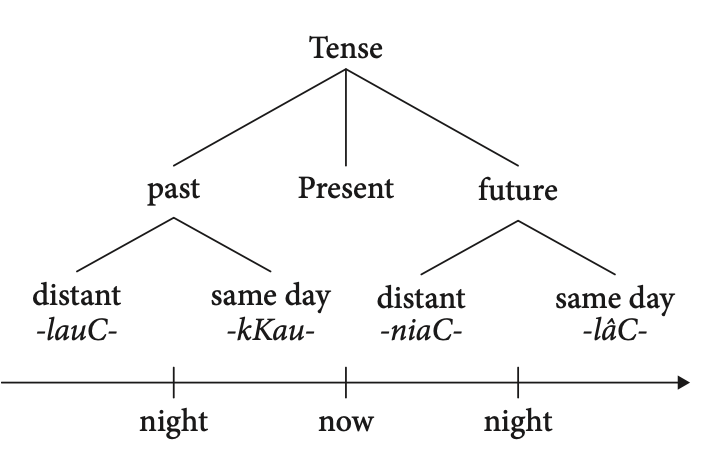
\includegraphics[height=5cm,width=8cm]{figures/SL1.png}
    \begin{forest} for tree = {fit=band}
		[tense, calign=child, calign child=2
			[past,name=past
				[distant\\
				 \textit{-lauC-}, align=center]
				[same day\\
				 \textit{-kKau-}, align=center]
			]
			[present,name=present]
			[future,name=future
				[distant\\
				 \textit{-niaC-},align=center]
				[same day\\
				 \textit{-lâC-}]
			]
		]
		\begin{scope}[every node/.style={inner sep=0pt, circle, fill=black, minimum size=5pt}]
		\node [below=2cm of past, label={below:{\strut night}}] (night) {};
		\node [below=2cm of present, label={below:{\strut now}}] (now) {};
		\node [below=2cm of future, label={below:{\strut night}}] (night2) {};
		\end{scope}
		\path let \p1=(current bounding box.west), \p2=(night) in node at (\x1,\y2) (leftanchor) {};
		\path let \p1=(current bounding box.east), \p2=(night) in node at (\x1,\y2) (rightanchor) {};
		\draw[-{Triangle[]}] (leftanchor) -- (night) -- (night2) -> (rightanchor);
	\end{forest}
    \caption{Semantic tense features in “full” Labrador Inuttitut}
    \label{SL1}
\end{figure}

\noindent
Contrast this situation with the feature inventory presents in “heritage” Labrador Inuttitut \citep[44]{sherkinalieber2015} in Figure \ref{SL2}.

\begin{figure}
% %     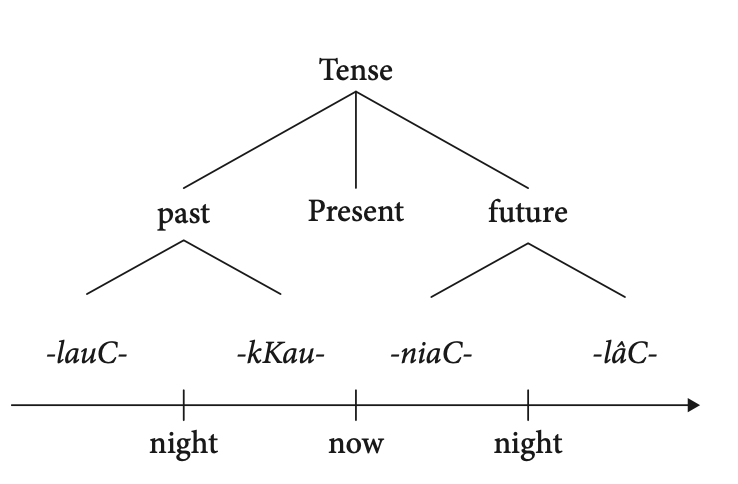
\includegraphics[height=5cm,width=8cm]{figures/SH2.png}
    	\begin{forest} for tree = {fit=band}
		[tense, calign=child, calign child=2
			[past,name=past
				[\textit{-lauC-}]
				[\textit{-kKau-}]
			]
			[present,name=present]
			[future,name=future
				[\textit{-niaC-}]
				[\textit{-lâC-}]
			]
		]
		\begin{scope}[every node/.style={inner sep=0pt, circle, fill=black, minimum size=5pt}]
		\node [below=1.25cm of past, label={below:{\strut night}}] (night) {};
		\node [below=1.25cm of present, label={below:{\strut now}}] (now) {};
		\node [below=1.25cm of future, label={below:{\strut night}}] (night2) {};
		\end{scope}	
		\path let \p1=(current bounding box.west), \p2=(night) in node at (\x1,\y2) (leftanchor) {};
		\path let \p1=(current bounding box.east), \p2=(night) in node at (\x1,\y2) (rightanchor) {};
		\draw[-{Triangle[]}] (leftanchor) -- (night) -- (night2) -> (rightanchor);
	\end{forest}
    \caption{Semantic tense features in “heritage” Labrador Inuttitut}
    \label{SL2}
\end{figure}

Comparing the feature inventories of the “full” and “heritage” variants with one another, we see that each tense morpheme is specified for both time and remoteness, whereas in the heritage speakers, each tense morpheme only has a specification for time. That is, no information about remoteness is available. That means that even if these speakers have two markers for each tense available, they are not able to distinguish them. As \citet[45]{sherkinalieber2015} points out, remoteness is likely to be vulnerable due to a lack of any analogue in English. Features of a weaker language which have no counterpart in the dominant language tend to be more vulnerable across heritage languages. Here we also see generalized exponence at work: There are two morphemes available that are no longer associated with an underlying feature distinction. In that sense, the morphemes contain fewer features, even though the number of exponents remains the same.

As for Cherokee, we observe the application of the 3rd plural prenominal prefixes in all environments, which represents a prototypical case of \textit{overgeneralization}. That is, speakers are no longer sensitive to verbs taking different prefixes. Again we see a case of generalized exponence where speakers are no longer sensitive to a distinction that exists in the baseline. That is, the distinction between Vocabulary Insertion rules in (\ref{distinction}) is eliminated and speakers instead adopt the rule in (\ref{nodistinction}). For expository convenience, we have just utilized a binary feature [\pm A] to refer to the distinction between Set A and Set B.

\begin{exe}
\ex\label{distinction} 
\begin{xlist}
\ex $[$\textsc{number:plural, person: 3, +A}$]$ $\Longleftrightarrow$ {\itshape ani-}
\ex $[$\textsc{number:plural, person: 3, −A}$]$ $\Longleftrightarrow$ {\itshape uni-}
\end{xlist}
\ex\label{nodistinction} $[$\textsc{number:plural, person: 3}$]$ $\Longleftrightarrow$ {\itshape ani-}
\end{exe}

\noindent
In addition, as described above, some speakers also use the singular prefix as opposed to the plural, possibly indicating the beginning of a merger of the singular and plural pronominal prefixes.

Turning to the definiteness system in American Hungarian, we see that definiteness marking in this particular heritage language appears to have been “simplified”. This difference, when compared to the baseline of European Hungarian, can be viewed as yet another instance of \textit{generalized exponence}, in the sense that speakers try to unify agreement within a minimal domain (viz. the nominal phrase in this case).

American Hungarian also lacks obligatory verbalizers in the speech of child bilinguals, or at the very least, the verbalizers are mastered only after the age of six. Theoretically, this is an interesting case, especially from the perspective of Distributed Morphology. Recall, that roots exist in the lexicon as a-categorial, featureless that receive categorial status by virtue of merging with a categorizer in the syntax. An illustration of this is provided in examples (\ref{roots}--\ref{roots2}) for nouns and verbs, respectively.

\begin{multicols}{2}

\begin{exe}
\ex \label{roots}
 \Tree [.\textit{n}P \textit{n} $\sqrt{\text{root}}$ ]
\end{exe}

\columnbreak

\begin{exe}
\ex \label{roots2}
\Tree [.\textit{v}P \textit{v} $\sqrt{\text{root}}$ ]
\end{exe}

\end{multicols}


In many languages, such categorizers have overt exponents. This can easily be seen in English, where morphemes such as {\itshape -en, -age, -al} realize the categorizers {\itshape v, n} and {\itshape a} for words such as {\itshape darken, marriage, global}. In \sectref{weaksub}, we saw that American Hungarian shows the tendency of not retaining these obligatory verbalizers as anticipated in instances of language-mixing. By assumption, such categorizing heads are present early on in acquisition. This state of affairs means that for some reason American Hungarian speakers are tolerating what is effectively a “silent” head for some time, at least throughout some stages of development. This behavior at first glance appears to contradict an established claim in the heritage language literature arguing that heritage speakers struggle with silence, i.e., elements in syntactic structure that do not map to a corresponding phonological exponent in general (see \citet{polinsky2018heritage} for an extensive review), but this difference highlights the importance of also considering typologically diverse languages when crafting generalizations.

To illustrate how we would formalize this situation, consider example (\ref{vbzexamples}a), repeated below as (\ref{xxx}):


\begin{exe}

\ex \gll \textit{cover}-\textbf{ol}-ja \\
          cover-\textsc{\textbf{vbz}-pres.3sg.def} \\
          \glt `[it] covers [it]' \label{xxx}

\end{exe}

The verbalizing exponent \textit{-ol-} in (\ref{xxx}) is the morphophonological manifestation of the categorizing head \textit{v}. The tree structure in (\ref{roots22}) immediately below holds for American Hungarian expressions which contain and omit this verbalizing exponent.

\begin{exe}
\ex \label{roots22}
\Tree [.Def {[+\textsc{def}]}
      [.Num 3\textsc{sg} 
      [.\textit{v}P \textit{v} $\sqrt{\text{root}}$ ] ] ]
\end{exe}

\noindent
While the features [+\textsc{def}] and 3\textsc{sg} undergo fusion and are spelled out as \textit{ja} in (\ref{xxx}), the Vocabulary Items for \textit{v} are optional, at least in a developmental sense: 

\begin{exe}
\ex\label{spellingoutv} 
\begin{xlist}
\ex $[\textit{v}\,]$ $\Longleftrightarrow$ {\itshape ol} \hfill[Overt realization of \textit{v}]
\ex $[\textit{v}\,]$ $\Longleftrightarrow$ ∅ \hfill[Non-realization of \textit{v}]
\end{xlist}

\end{exe}


Another puzzle that emerges in connection with American Hungarian concerns the inclusion of additional proforms. On the one hand, we are dealing with one-to-one mappings, which we have argued are simpler than one-to-many mappings. However, this also leads to (i) redundancy, and (ii) the realization of smaller units (proforms) as “independent units” that used to be realized as suffixes. Classifying the occurrence of the realization of these (additional) proforms in terms of either reduced or increased complexity is quite difficult, but based on the decomposition  of syntactic structures and their morphological reflexes proposed in \sectref{formalcomplexity}, we adopt the position that these mappings result in more straightforward instances of correspondence, even if they ultimately lead to redundancy and additional independent units. This may be an instance of what \citet{maximizexp} call \textsc{maximize exponence} (\ref{maxexp}), which holds that for each semantic feature at least one exponent should be realized. Their evidence come from a very different empirical domain, and, with converging evidence from multiple speaker groups, this suggests that we are dealing with a possibly deep generalization regarding the interface between features and exponents.

Lastly, we provide a few remarks on instances of divergent preverb placement in American Hungarian. Recall from our discussion of the data in (\ref{bol1}) that whereas the preverbal particle \textit{meg} raises to precede the auxiliary in European Hungarian, this fails to leave the verbal phrase in American Hungarian, appearing as a proclitic to the lexical verb. This situation illustrates the potential reduction in the movement of this preverbal particle, which can further be generalized to be a reduction in the computational domain of movement, i.e., a “minimal domain” effect. The latter has been demonstrated also in other cases, for instance long-distance binding \citep{gurel2007, kimetal2009, mikebirna2015, Montrul2016} and A-bar dependencies \citep{hoppetalwh}. Further research should examine to what extend these “minimal domain” effects can be equated with some version of phase theory (see, e.g., \citealt{chomsky2000, chomsky2001, gallego2010}), which is a fruitful topic that we leave for future inquiry.

Let us return to the typology proposed by \citet{lohnput21} in connection with an exoskeletal approach to complexity at the morphology-syntax interface, repeated in (\ref{no11}) for expository convenience.

\begin{exe}
\ex\label{no11} Relative to a given baseline, a feature can
\begin{xlist}
        \item be retained in the same hierarchical position
        \item shift its hierarchical position
        \item be lost
        \item be (internally) restructured through
        \begin{xlist}
        \item loss of (some) features
        \item reconfiguration of features
        \end{xlist}
\end{xlist}
\end{exe}

The data reviewed in \sectref{verbsection} provide evidence for (\ref{no11}d) and illustrate how some features and feature distinctions can be lost or eliminated. In order to better understand the mapping from features to exponents, we have focused on what we have called \textit{generalized exponence}, which illustrates a situation where heritage speakers use an exponent in more contexts than baseline speakers. It should be added that generalized exponence can often be found in situations of language change more generally, although space prevents us from addressing that issue here.

Zooming out, the data and analyses in this chapter suggest that the particular morphological type is not a decisive factor when it comes to decomposing complexity in heritage languages. The same basic mechanisms appear to be at work across morphological systems. As such, this aligns with the generalizations and conclusions arrived at in \citet{putnametal2021}; namely, that irrespective of the morphological typology of a given language, or dyad of languages in the case of heritage speakers, similar patterns of morphological outputs in heritage languages will manifest themselves along the lines of the five tendencies outlined in \sectref{common}. Theoretically, these data adduce further support for a late-insertion account of morphology whereby the syntactic features are independent of morphophonological exponents. The review of different approaches to the syntax-morphology interface in \sectref{formalcomplexity} demonstrates that even within late insertion approaches there are substantial differences. The data in the present chapter can easily be analyzed within Distributed Morphology.\footnote{They are also compatible with a Nanosyntactic account, although as far as we can tell, the data do not appear to necessitate such an approach.}


\section{Conclusion} \label{outro}\largerpage[2]
Our main purpose in this chapter was to unite current theoretical analyses of heritage language morphology with discussions centered on notions of \textit{complexity} in heritage languages (and linguistic systems more generally). For the sake of space and time, we zeroed in on two empirical phenomena found in agglutinating languages, namely, \textit{increased analyticity} and \textit{generalized exponency}. Unsurprisingly, these heritage languages show an increased amount of one-to-one mappings (\textit{increased analyticity}) and a reduction in feature-exponent mappings (\textit{generalized exponency}), as explicated in detailed reviews by \citet[Ch.5]{polinsky2018heritage} and \citet{putnametal2021}. Interpreting these findings through the lens of an exoskeletal approach to the morphology-syntax interface as laid out by \citet{lohnput21} (see \sectref{formalcomplexity}), three primary outcomes emerge: First, the relative size of syntactic objects appears to be somewhat larger in heritage language morphosyntax. That is, the units that are lexicalized are larger because of changes in the feature structure. Under this notion, the semantic content of some features that were associated with morphophonological exponency is \textit{weakened}, leading to the eventual possible loss of these connections. Therefore, whereas the syntactic objects, i.e., the domains of syntactic structure that are lexicalized, may grow in size, the inventory of exponents they may be associated with may be (significantly) reduced. In some respects, we witness a “hollowing out” of syntactic structure, which forces us to revisit exactly what “representational economy” \citep{scontras2015,ScontrasEtAl2018,PolinskyScontras2020} means in the context of the morphology-syntax interface in heritage languages. Second, instances of \textit{overmarking} and \textit{redundancy} sometimes accompany the observable trend toward analyticity. Even if such structures represent a transient state of the heritage language grammar, they represent instances of \textit{distributed exponency}, which reinforce that not all morphological developments in heritage languages can be interpreted as internally-motivated simplification strategies \citep{bousquette2020}. Third, the reduction in computational domains with respect to potential spell-out domains plays a role in the appearance of this aforementioned distributed exponency, as well as in the obfuscation of preverbal marker placement in languages such as American Hungarian. 

The next frontier would be to see how the ideas in this chapter extend to other agglutinating and polysynthetic languages, in particular the latter. Although studies on “obsolescence” in polysynthetic languages appear to exhibit similar morphological patterns \citep{mithun1989incipient,gruzdeva&vakhtin2017}, the interplay of complex phonological alternations adds yet an additional important, yet intriguing domain to the puzzle of systemic complexity in heritage languages.


%\section*{Extra stuff from template}

%\begin{table}[h!]
%\caption{Frequencies of word classes}
%\label{tab:1:frequencies}
% \begin{tabular}{l rrrr}
%  \lsptoprule
%            & nouns & verbs  & adjectives & adverbs\\
%  \midrule
%  absolute  &   12  &    34  &    23      & 13\\
%  relative  &   3.1 &   8.9  &    5.7     & 3.2\\
%  \lspbottomrule
% \end{tabular}
%\end{table}

%\is{Cognition} %add "Cogntion" to subject index for this page

%\ea
%\gll cogito                           ergo      sum\\
%     think.\textsc{1sg}.\textsc{pres} therefore %\textsc{cop}.\textsc{1sg}.\textsc{pres}\\
%\glt `I think therefore I am.'
%\z
%\il{Latin} %add "Latin" to language index for this page

%\textcolor{red}{\textbf{Probably not gonna keep this...}}
%In Hungarian, verbal inflection marks agreement with both the subject and the object. They are can be realized as either portmanteau or separate inflection. Similar to English, in Hungarian the verb displays person and number agreement with the subject; however, in contrast to English, there is no morphological plural agreement when the the subject phrase contains either (i) a numeral or (ii) a quantifier. Nouns also are not marked for plural in Hungarian, which is only indicated by the semantics of the plural or quantifier. 

%\begin{exe}

%\ex \gll Sok vend\'{e}g \'{e}rkez-ett. \\
%         many guest-\textsc{sg.nom} arrive-\textsc{past.3sg.indef} \\
%         \glt `Many guests have arrived.' \label{HungSVagr}

%\end{exe}

%\noindent
% The verb agrees with the object with respect to (in)definiteness and specificity in Hungarian object-verb agreement. Two separate paradigms are utilized to distinguish between \textit{indefinite} and \textit{definite} conjugations. This is illustrated in (\ref{HungOVagr}) below; with the indefinite conjugation appearing in (\ref{HungOVagr}a) and the definite in (\ref{HungOVagr}b). 
 
% \begin{exe}
% \ex \label{HungOVagr}
%\begin{xlist}
% \ex \gll (Én) lát-\textbf{ok} egy kalap-ot. \\
%            (I) see-\textsc{pres.1sg.indef} a hat-\textsc{acc} \\
%     \glt `I see a hat.' 

%\ex \gll (Én) lát-\textbf{om} a kalap-ot. \\
%         (I) see-see-\textsc{pres.1sg.def} the hat-\textsc{acc} \\
%        \glt  `I see the hat.' 
 
%\end{xlist}
% \end{exe}


\section*{Abbreviations}\largerpage
\begin{multicols}{2}
\begin{tabbing}
\textsc{supresss} \=  supressive  \kill
\textsc{a} \>        Set A  \\
\textsc{dat} \>      dative  \\
\textsc{def} \>      definite  \\
\textsc{delat} \>    delative  \\
\textsc{dpst} \>     distant past  \\
\textsc{dst} \>      distributive  \\
\textsc{impfv} \>    imperfective  \\
\textsc{ind} \>      indicative  \\
\textsc{indef} \>    indefinite  \\
\textsc{inf} \>      infinitive  \\
\textsc{obj} \>      object (non-agentive)  \\
\textsc{part} \>     partitive  \\
\textsc{pl} \>       plural  \\
\textsc{poss} \>     possessive  \\
\textsc{prc} \>      progressive  \\
\textsc{pres} \>     present tense  \\
\textsc{pst} \>      past tense  \\
\textsc{pvb} \>      preverbal element  \\
\textsc{sg} \>       singular  \\
\textsc{supress} \>  supressive  \\
\textsc{vbz} \>      verbalizer  \\
\end{tabbing}
\end{multicols}

\section*{Acknowledgments}
Thanks are in order to Artemis Alexiadou for reading through and commenting on a final version of this chapter. We also owe a debt of gratitude to an anonymous reviewer for their challenging and probing questions and criticisms which ultimately strengthened this chapter. A special thanks to David Natvig and Ashley Pahis for some \LaTeX{} troubleshooting. 

\printbibliography[heading=subbibliography,notkeyword=this]

\end{document} 
